\documentclass[notheorems]{beamer}

%Fuer Praesentationen mit einem Beamer sinnvolle Schriftenwahl fuer Text, Mathe und Verbatim
\usepackage[scaled=.90]{helvet}
\usepackage{mathptmx}
\usepackage{courier}
\usepackage[english]{babel}
\usepackage[utf8]{inputenc}
\usepackage{geometry}
\usepackage{dsfont}
\usepackage{ mathdots }
\usepackage{marvosym}
\usepackage{ stmaryrd }
\usepackage{xspace}
\usepackage{verbatim}
\usepackage{amssymb, amsthm}
\usepackage[margin=10pt,font=small,labelfont=bf]{caption}
\usepackage{amsmath}
\usepackage{tikz}
\usetikzlibrary{trees,automata,arrows,shapes}
\usepackage{amsfonts}
\usepackage{xcolor}
\usepackage{hyperref}
\usepackage{graphicx}
\usepackage{framed}
\usepackage{ifthen}
\usepackage{xcolor}
\usetikzlibrary{calc,patterns,angles,quotes}
\theoremstyle{plain}
\newtheorem{thrm}{Theorem}
\newtheorem{prop}{Lemma}
\newtheorem{property}{Property}
\newtheorem{rem}{Remark}
\newtheorem{prof}{Proof}
\newtheorem{contProof}{Proof Continuation}
\newtheorem{problem}{Problem}

\theoremstyle{definition}
\newtheorem{defn}{Definition}
\newtheorem{con}{Conjecture}
\newtheorem{example}{Example}
\colorlet{shadecolor}{orange!15}
\newenvironment{exmp}
	{\begin{shaded}\begin{example}}
	{\end{example}\end{shaded}}
\theoremstyle{remark}
\newtheorem{exkurs}{Exkurs}
\newenvironment{ex}
	{\begin{shaded}\begin{exkurs}}
	{\end{exkurs}\end{shaded}}

%Grundthema waehlen, evtl. mit den anderen Theme-Befehlen veraendern
\usetheme{Warsaw}
\usecolortheme{dolphin}
\usefonttheme{serif}
%\useinnertheme{rectangles}
\useoutertheme{infolines}


%Overlays sind nicht ganz unsichtbar, sondern schwach im Hintergrund zu sehen solange sie noch nicht aufgedeckt sind
\setbeamercovered{transparent}
\setbeamertemplate{bibliography item}{\insertbiblabel}

%keine Navigationssymbole unten rechts anzeigen
\beamertemplatenavigationsymbolsempty
%\setbeamertemplate{navigation symbols}{}
\definecolor{darkblue}{RGB}{132,112,255}
%\logo{\includegraphics[width=1cm]{emblem_rainbow.jpg}}
%\titlegraphic{\includegraphics[width=1cm]{emblem_rainbow.jpg}}

\newcommand{\dist}[1]{\ensuremath\text{d}\left(#1\right)}

\begin{document}

\frame{
	\frametitle{Outline}
	\tableofcontents
%um Pausen zwischen den sections beim Vorlesen der Uebersicht zu erzeugen
%	[pausesections]
}

\section{Contest Problem}
%\subsection{Scope}
%\frame{
%	\frametitle{}
%	\begin{itemize}
%	\item Characterisation of Planar Graphs: Introduction of planar graphs.
%	\item<2,3,4,5> Characterisation of IC-planar Graphs: Characterisation of IC-planar graphs and its relationship to planar graphs.
%	\item<3,4,5> Drawing IC-planar Graphs: How to draw such an graph efficiently?
%	\item<4,5> IC-Planarity Testing: Is a given graph IC-planar?
%	\item<5> Coloring IC-planar graphs: What is the bound of the chromatic number on IC-planar graphs?
%	\end{itemize}
%}

\subsection{What is the problem of the contest?}
\frame{
	\frametitle{Minimizing the Crossing Angle}
}
\subsection{Classic spring embedder / BIGANGLE}
\begin{frame}{General idea}
\begin{itemize}
\item Calculate force for each node
\item Try to bring the graph into a minimum energy state
\item Assume time discrete 
\item[$\implies$] Each time step until convergence, add force vectors to node positions
\end{itemize}
\end{frame}
\begin{frame}{Forces}
$G = (V, E)$
\begin{itemize}
\item Nodes are charged particles 
$$\implies f_{el}(n_1, n_2) = \frac{\epsilon_{el}}{\dist{n_1, n_2}}~~\forall n_1, n_2\in V$$
\item Edges are springs 
$$\implies f_{sp}(n_1, n_2) = \epsilon_{sp}\cdot(\dist{n_1, n_2} - l_{sp})~~\forall e=(n_1, n_2)\in E$$
\item Increase crossing angles 
$$\implies f_{cr}(\vec{e_1}, \vec{e_2}, \theta) = (\hat{e_1}, \hat{e_2})\cdot\epsilon_{cr}\cos(\theta)~~\forall e_1, e_2\in \text{Crossings}\subseteq E\times E$$
\item Evenly distribute edges around nodes 
$$f_{n_1}(n_2, n_3, \phi)=\epsilon_{nb}\cdot\sin\left(\frac{\phi-\theta}2\right)~~\forall n_1\in V, n_2, n_3\in\text{Neighbours}(n_1)$$
\end{itemize}
\end{frame}
\begin{frame}{Problems and solutions}
\begin{itemize}
\item For large graphs this produces small drawings
\item Springs are too inflexible
$$l \sim \log(|N|), ~~ \epsilon_{sp}' = \frac{\dist{n_1, n_2} - l}l$$
$$\implies f_{sp}'(n_1, n_2) = \epsilon_{sp}'\cdot\tan^{-1}\left({\epsilon_{sp}'}^4\right);~~\forall e=(n_1, n_2)\in E$$
\item Spring embedder converges to local minimum
\item[$\implies$] Change embedding locally, keep good changes
\item[$\implies$] Genetic algorithm
\end{itemize}
\end{frame}
\begin{frame}{Mutation strategies}
\begin{itemize}
\item Change parameters of forces 
\item Exchange force variants
\item Remove crossing with worst crossing angle by swapping node positions
\end{itemize}
\end{frame}
\frame{
	\frametitle{Gridding the graph}\begin{center}
	
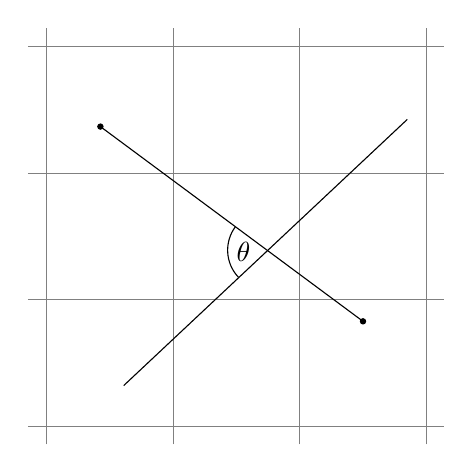
\begin{tikzpicture}[-, node distance=1.5cm,main node/.style={minimum size = .2cm,circle,draw, fill, scale=0.2}, scale=2.3, node/.style={scale=0.1}]  
\node[node] (1) at (0.887,1.22) {};
\node[main node] (2) at (1.75,0.58) {};
\node[node] (3) at (0.423,0.22) {};
\node[node] (4) at (2,1.7) {};
\node[node] (5) at (1.22,0.973) {};
\node[main node] (6) at (0.3, 1.6553) {};
\draw [step=0.7,gray, very thin] (-0.1,-0.1) grid (2.2,2.2);
\pic [draw, -, "$\theta$"] {angle = 1--5--3};
\path 
(6) edge (2)
(3)edge (4);
\end{tikzpicture}
	\end{center}

}

\frame{
	\frametitle{Four possibilities}
	\begin{center}
	\begin{minipage}[c]{0.3\textwidth}
	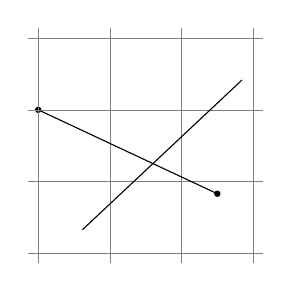
\begin{tikzpicture}[-, node distance=1.5cm,main node/.style={minimum size = .2cm,circle,draw, fill, scale=0.2}, scale=1.3, node/.style={scale=0.1}]  
\node[node] (1) at (0.887,1.22) {};
\node[main node] (2) at (1.75,0.58) {};
\node[node] (3) at (0.423,0.22) {};
\node[node] (4) at (2,1.7) {};
\node[node] (5) at (1.22,0.973) {};
\node[main node] (6) at (0.0, 1.4) {};
\draw [step=0.7,gray, very thin] (-0.1,-0.1) grid (2.2,2.2);
\path 
(6) edge (2)
(3)edge (4);
\end{tikzpicture} \\
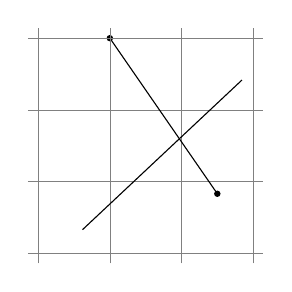
\begin{tikzpicture}[-, node distance=1.5cm,main node/.style={minimum size = .2cm,circle,draw, fill, scale=0.2}, scale=1.3, node/.style={scale=0.1}]  
\node[node] (1) at (0.887,1.22) {};
\node[main node] (2) at (1.75,0.58) {};
\node[node] (3) at (0.423,0.22) {};
\node[node] (4) at (2,1.7) {};
\node[node] (5) at (1.22,0.973) {};
\node[main node] (6) at (0.7, 2.1) {};
\draw [step=0.7,gray, very thin] (-0.1,-0.1) grid (2.2,2.2);
\path 
(6) edge (2)
(3)edge (4);
\end{tikzpicture}
	\end{minipage}~
	\begin{minipage}[c]{0.3\textwidth}
	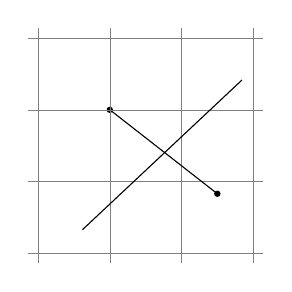
\begin{tikzpicture}[-, node distance=1.5cm,main node/.style={minimum size = .2cm,circle,draw, fill, scale=0.2}, scale=1.3, node/.style={scale=0.1}]  
\node[node] (1) at (0.887,1.22) {};
\node[main node] (2) at (1.75,0.58) {};
\node[node] (3) at (0.423,0.22) {};
\node[node] (4) at (2,1.7) {};
\node[node] (5) at (1.22,0.973) {};
\node[main node] (6) at (0.7, 1.4) {};
\draw [step=0.7,gray, very thin] (-0.1,-0.1) grid (2.2,2.2);
\path 
(6) edge (2)
(3)edge (4);
\end{tikzpicture} \\
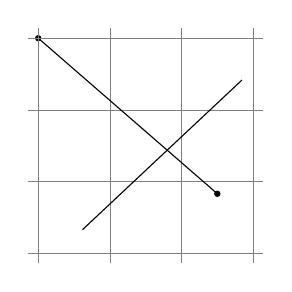
\begin{tikzpicture}[-, node distance=1.5cm,main node/.style={minimum size = .2cm,circle,draw, fill, scale=0.2}, scale=1.3, node/.style={scale=0.1}]  
\node[node] (1) at (0.887,1.22) {};
\node[main node] (2) at (1.75,0.58) {};
\node[node] (3) at (0.423,0.22) {};
\node[node] (4) at (2,1.7) {};
\node[node] (5) at (1.22,0.973) {};
\node[main node] (6) at (0.0, 2.1) {};
\draw [step=0.7,gray, very thin] (-0.1,-0.1) grid (2.2,2.2);
\path 
(6) edge (2)
(3)edge (4);
\end{tikzpicture}
	\end{minipage}
	\end{center}
}

\frame{
	\frametitle{Sixteen possibilities...}
	\begin{center}
	\begin{minipage}[c]{0.2\textwidth}
	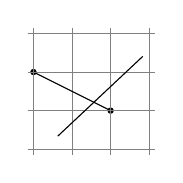
\begin{tikzpicture}[-, node distance=1.5cm,main node/.style={minimum size = .2cm,circle,draw, fill, scale=0.2}, scale=0.7, node/.style={scale=0.1}]  
\node[node] (1) at (0.887,1.22) {};
\node[main node] (2) at (1.4,0.7) {};
\node[node] (3) at (0.423,0.22) {};
\node[node] (4) at (2,1.7) {};
\node[node] (5) at (1.22,0.973) {};
\node[main node] (6) at (0.0, 1.4) {};
\draw [step=0.7,gray, very thin] (-0.1,-0.1) grid (2.2,2.2);
\path 
(6) edge (2)
(3)edge (4);
\end{tikzpicture} \\
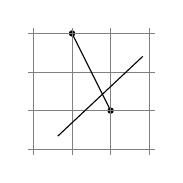
\begin{tikzpicture}[-, node distance=1.5cm,main node/.style={minimum size = .2cm,circle,draw, fill, scale=0.2}, scale=0.7, node/.style={scale=0.1}]  
\node[node] (1) at (0.887,1.22) {};
\node[main node] (2) at (1.4,0.7) {};
\node[node] (3) at (0.423,0.22) {};
\node[node] (4) at (2,1.7) {};
\node[node] (5) at (1.22,0.973) {};
\node[main node] (6) at (0.7, 2.1) {};
\draw [step=0.7,gray, very thin] (-0.1,-0.1) grid (2.2,2.2);
\path 
(6) edge (2)
(3)edge (4);
\end{tikzpicture} \\
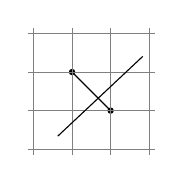
\begin{tikzpicture}[-, node distance=1.5cm,main node/.style={minimum size = .2cm,circle,draw, fill, scale=0.2}, scale=0.7, node/.style={scale=0.1}]  
\node[node] (1) at (0.887,1.22) {};
\node[main node] (2) at (1.4,0.7) {};
\node[node] (3) at (0.423,0.22) {};
\node[node] (4) at (2,1.7) {};
\node[node] (5) at (1.22,0.973) {};
\node[main node] (6) at (0.7, 1.4) {};
\draw [step=0.7,gray, very thin] (-0.1,-0.1) grid (2.2,2.2);
\path 
(6) edge (2)
(3)edge (4);
\end{tikzpicture} \\
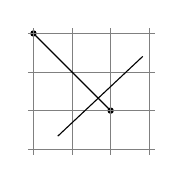
\begin{tikzpicture}[-, node distance=1.5cm,main node/.style={minimum size = .2cm,circle,draw, fill, scale=0.2}, scale=0.7, node/.style={scale=0.1}]  
\node[node] (1) at (0.887,1.22) {};
\node[main node] (2) at (1.4,0.7) {};
\node[node] (3) at (0.423,0.22) {};
\node[node] (4) at (2,1.7) {};
\node[node] (5) at (1.22,0.973) {};
\node[main node] (6) at (0.0, 2.1) {};
\draw [step=0.7,gray, very thin] (-0.1,-0.1) grid (2.2,2.2);
\path 
(6) edge (2)
(3)edge (4);
\end{tikzpicture}
	\end{minipage}~
	\begin{minipage}[c]{0.2\textwidth}
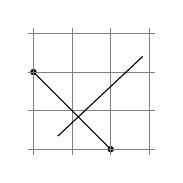
\begin{tikzpicture}[-, node distance=1.5cm,main node/.style={minimum size = .2cm,circle,draw, fill, scale=0.2}, scale=0.7, node/.style={scale=0.1}]  
\node[node] (1) at (0.887,1.22) {};
\node[main node] (2) at (1.4,0.0) {};
\node[node] (3) at (0.423,0.22) {};
\node[node] (4) at (2,1.7) {};
\node[node] (5) at (1.22,0.973) {};
\node[main node] (6) at (0.0, 1.4) {};
\draw [step=0.7,gray, very thin] (-0.1,-0.1) grid (2.2,2.2);
\path 
(6) edge (2)
(3)edge (4);
\end{tikzpicture} \\
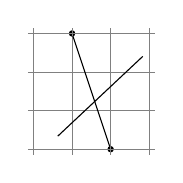
\begin{tikzpicture}[-, node distance=1.5cm,main node/.style={minimum size = .2cm,circle,draw, fill, scale=0.2}, scale=0.7, node/.style={scale=0.1}]  
\node[node] (1) at (0.887,1.22) {};
\node[main node] (2) at (1.4,0.0) {};
\node[node] (3) at (0.423,0.22) {};
\node[node] (4) at (2,1.7) {};
\node[node] (5) at (1.22,0.973) {};
\node[main node] (6) at (0.7, 2.1) {};
\draw [step=0.7,gray, very thin] (-0.1,-0.1) grid (2.2,2.2);
\path 
(6) edge (2)
(3)edge (4);
\end{tikzpicture} \\
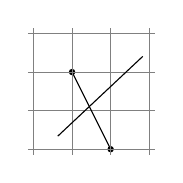
\begin{tikzpicture}[-, node distance=1.5cm,main node/.style={minimum size = .2cm,circle,draw, fill, scale=0.2}, scale=0.7, node/.style={scale=0.1}]  
\node[node] (1) at (0.887,1.22) {};
\node[main node] (2) at (1.4,0.0) {};
\node[node] (3) at (0.423,0.22) {};
\node[node] (4) at (2,1.7) {};
\node[node] (5) at (1.22,0.973) {};
\node[main node] (6) at (0.7, 1.4) {};
\draw [step=0.7,gray, very thin] (-0.1,-0.1) grid (2.2,2.2);
\path 
(6) edge (2)
(3)edge (4);
\end{tikzpicture} \\
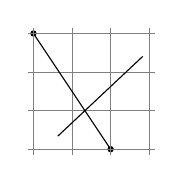
\begin{tikzpicture}[-, node distance=1.5cm,main node/.style={minimum size = .2cm,circle,draw, fill, scale=0.2}, scale=0.7, node/.style={scale=0.1}]  
\node[node] (1) at (0.887,1.22) {};
\node[main node] (2) at (1.4,0.0) {};
\node[node] (3) at (0.423,0.22) {};
\node[node] (4) at (2,1.7) {};
\node[node] (5) at (1.22,0.973) {};
\node[main node] (6) at (0.0, 2.1) {};
\draw [step=0.7,gray, very thin] (-0.1,-0.1) grid (2.2,2.2);
\path 
(6) edge (2)
(3)edge (4);
\end{tikzpicture}
	\end{minipage}
		\begin{minipage}[c]{0.2\textwidth}
	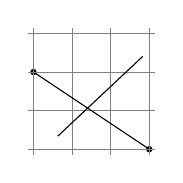
\begin{tikzpicture}[-, node distance=1.5cm,main node/.style={minimum size = .2cm,circle,draw, fill, scale=0.2}, scale=0.7, node/.style={scale=0.1}]  
\node[node] (1) at (0.887,1.22) {};
\node[main node] (2) at (2.1,0.0) {};
\node[node] (3) at (0.423,0.22) {};
\node[node] (4) at (2,1.7) {};
\node[node] (5) at (1.22,0.973) {};
\node[main node] (6) at (0.0, 1.4) {};
\draw [step=0.7,gray, very thin] (-0.1,-0.1) grid (2.2,2.2);
\path 
(6) edge (2)
(3)edge (4);
\end{tikzpicture} \\
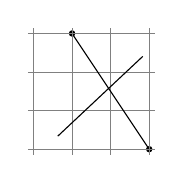
\begin{tikzpicture}[-, node distance=1.5cm,main node/.style={minimum size = .2cm,circle,draw, fill, scale=0.2}, scale=0.7, node/.style={scale=0.1}]  
\node[node] (1) at (0.887,1.22) {};
\node[main node] (2) at (2.1,0.0) {};
\node[node] (3) at (0.423,0.22) {};
\node[node] (4) at (2,1.7) {};
\node[node] (5) at (1.22,0.973) {};
\node[main node] (6) at (0.7, 2.1) {};
\draw [step=0.7,gray, very thin] (-0.1,-0.1) grid (2.2,2.2);
\path 
(6) edge (2)
(3)edge (4);
\end{tikzpicture} \\
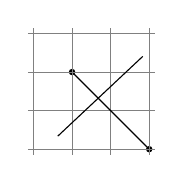
\begin{tikzpicture}[-, node distance=1.5cm,main node/.style={minimum size = .2cm,circle,draw, fill, scale=0.2}, scale=0.7, node/.style={scale=0.1}]  
\node[node] (1) at (0.887,1.22) {};
\node[main node] (2) at (2.1,0.0) {};
\node[node] (3) at (0.423,0.22) {};
\node[node] (4) at (2,1.7) {};
\node[node] (5) at (1.22,0.973) {};
\node[main node] (6) at (0.7, 1.4) {};
\draw [step=0.7,gray, very thin] (-0.1,-0.1) grid (2.2,2.2);
\path 
(6) edge (2)
(3)edge (4);
\end{tikzpicture} \\
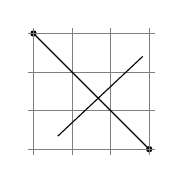
\begin{tikzpicture}[-, node distance=1.5cm,main node/.style={minimum size = .2cm,circle,draw, fill, scale=0.2}, scale=0.7, node/.style={scale=0.1}]  
\node[node] (1) at (0.887,1.22) {};
\node[main node] (2) at (2.1,0.0) {};
\node[node] (3) at (0.423,0.22) {};
\node[node] (4) at (2,1.7) {};
\node[node] (5) at (1.22,0.973) {};
\node[main node] (6) at (0.0, 2.1) {};
\draw [step=0.7,gray, very thin] (-0.1,-0.1) grid (2.2,2.2);
\path 
(6) edge (2)
(3)edge (4);
\end{tikzpicture}
	\end{minipage}
	\begin{minipage}[c]{0.2\textwidth}
	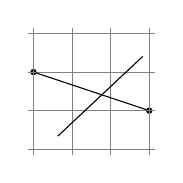
\begin{tikzpicture}[-, node distance=1.5cm,main node/.style={minimum size = .2cm,circle,draw, fill, scale=0.2}, scale=0.7, node/.style={scale=0.1}]  
\node[node] (1) at (0.887,1.22) {};
\node[main node] (2) at (2.1,0.7) {};
\node[node] (3) at (0.423,0.22) {};
\node[node] (4) at (2,1.7) {};
\node[node] (5) at (1.22,0.973) {};
\node[main node] (6) at (0.0, 1.4) {};
\draw [step=0.7,gray, very thin] (-0.1,-0.1) grid (2.2,2.2);
\path 
(6) edge (2)
(3)edge (4);
\end{tikzpicture} \\
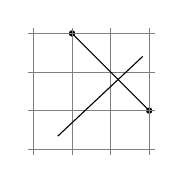
\begin{tikzpicture}[-, node distance=1.5cm,main node/.style={minimum size = .2cm,circle,draw, fill, scale=0.2}, scale=0.7, node/.style={scale=0.1}]  
\node[node] (1) at (0.887,1.22) {};
\node[main node] (2) at (2.1,0.7) {};
\node[node] (3) at (0.423,0.22) {};
\node[node] (4) at (2,1.7) {};
\node[node] (5) at (1.22,0.973) {};
\node[main node] (6) at (0.7, 2.1) {};
\draw [step=0.7,gray, very thin] (-0.1,-0.1) grid (2.2,2.2);
\path 
(6) edge (2)
(3)edge (4);
\end{tikzpicture} \\
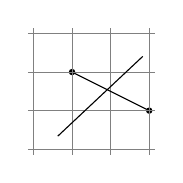
\begin{tikzpicture}[-, node distance=1.5cm,main node/.style={minimum size = .2cm,circle,draw, fill, scale=0.2}, scale=0.7, node/.style={scale=0.1}]  
\node[node] (1) at (0.887,1.22) {};
\node[main node] (2) at (2.1,0.7){};
\node[node] (3) at (0.423,0.22) {};
\node[node] (4) at (2,1.7) {};
\node[node] (5) at (1.22,0.973) {};
\node[main node] (6) at (0.7, 1.4) {};
\draw [step=0.7,gray, very thin] (-0.1,-0.1) grid (2.2,2.2);
\path 
(6) edge (2)
(3)edge (4);
\end{tikzpicture} \\
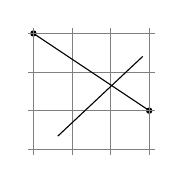
\begin{tikzpicture}[-, node distance=1.5cm,main node/.style={minimum size = .2cm,circle,draw, fill, scale=0.2}, scale=0.7, node/.style={scale=0.1}]  
\node[node] (1) at (0.887,1.22) {};
\node[main node] (2) at (2.1,0.7) {};
\node[node] (3) at (0.423,0.22) {};
\node[node] (4) at (2,1.7) {};
\node[node] (5) at (1.22,0.973) {};
\node[main node] (6) at (0.0, 2.1) {};
\draw [step=0.7,gray, very thin] (-0.1,-0.1) grid (2.2,2.2);
\path 
(6) edge (2)
(3)edge (4);
\end{tikzpicture}
	\end{minipage}
	\end{center}
}

\frame{
	\frametitle{Implementation of two algorithms}	
	\begin{itemize}
		\item Simple Gridding: Check for each vertex $v$ if creates new crossing with grid coordinates? \\
		\begin{center}
		\begin{minipage}[c]{0.3\textwidth}
		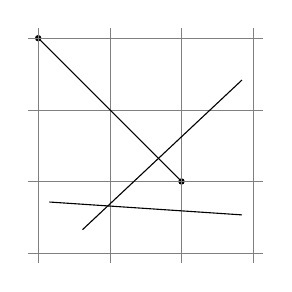
\begin{tikzpicture}[-, node distance=1.5cm,main node/.style={minimum size = .2cm,circle,draw, fill, scale=0.2}, scale=1.3, node/.style={scale=0.1}]  
\node[node] (1) at (0.887,1.22) {};
\node[main node] (2) at (1.4,0.7) {};
\node[node] (3) at (0.423,0.22) {};
\node[node] (4) at (2,1.7) {};
\node[node] (5) at (1.22,0.973) {};
\node[node] (7) at (0.1,0.5) {};
\node[node] (8) at (2,0.373) {};
\node[main node] (6) at (0.0, 2.1) {};
\draw [step=0.7,gray, very thin] (-0.1,-0.1) grid (2.2,2.2);
\path 
(6) edge (2)
(3)edge (4)
(7) edge (8);
\end{tikzpicture}\\
 \begin{center}
 \textcolor{green}{$\surd$}
 \end{center}
\end{minipage}	~
\begin{minipage}[c]{0.3\textwidth}
		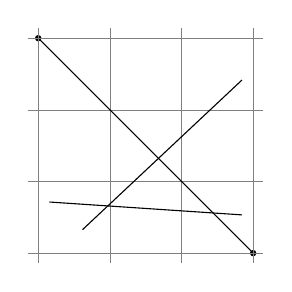
\begin{tikzpicture}[-, node distance=1.5cm,main node/.style={minimum size = .2cm,circle,draw, fill, scale=0.2}, scale=1.3, node/.style={scale=0.1}]  
\node[node] (1) at (0.887,1.22) {};
\node[main node] (2) at (2.1,0.0) {};
\node[node] (3) at (0.423,0.22) {};
\node[node] (4) at (2,1.7) {};
\node[node] (5) at (1.22,0.973) {};
\node[node] (7) at (0.1,0.5) {};
\node[node] (8) at (2,0.373) {};
\node[main node] (6) at (0.0, 2.1) {};
\draw [step=0.7,gray, very thin] (-0.1,-0.1) grid (2.2,2.2);
\path 
(6) edge (2)
(3)edge (4)
(7) edge (8);
\end{tikzpicture} \\
\begin{center}
\textcolor{red}{$\lightning$}
\end{center}
\end{minipage}			
		\end{center}
	\end{itemize}
}
\frame{
	\begin{itemize}	
		\item Non-Simple Gridding: Check for each vertex $v$ that minimum angle not compromissed!
				\begin{center}
		\begin{minipage}[c]{0.3\textwidth}
		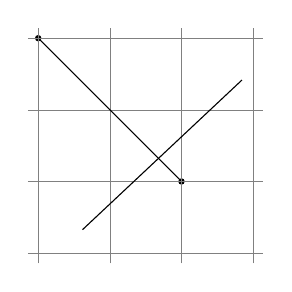
\begin{tikzpicture}[-, node distance=1.5cm,main node/.style={minimum size = .2cm,circle,draw, fill, scale=0.2}, scale=1.3, node/.style={scale=0.1}]  
\node[node] (1) at (0.887,1.22) {};
\node[main node] (2) at (1.4,0.7) {};
\node[node] (3) at (0.423,0.22) {};
\node[node] (4) at (2,1.7) {};
\node[node] (5) at (1.22,0.973) {};
\node[main node] (6) at (0.0, 2.1) {};
\draw [step=0.7,gray, very thin] (-0.1,-0.1) grid (2.2,2.2);
\path 
(6) edge (2)
(3)edge (4);
\end{tikzpicture}\\
 \begin{center}
 \textcolor{green}{$\surd$}
 \end{center}
\end{minipage}	~
\begin{minipage}[c]{0.3\textwidth}
		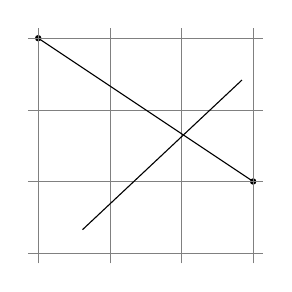
\begin{tikzpicture}[-, node distance=1.5cm,main node/.style={minimum size = .2cm,circle,draw, fill, scale=0.2}, scale=1.3, node/.style={scale=0.1}]  
\node[node] (1) at (0.887,1.22) {};
\node[main node] (2) at (2.1,0.7) {};
\node[node] (3) at (0.423,0.22) {};
\node[node] (4) at (2,1.7) {};
\node[node] (5) at (1.22,0.973) {};
\node[main node] (6) at (0.0, 2.1) {};
\draw [step=0.7,gray, very thin] (-0.1,-0.1) grid (2.2,2.2);
\path 
(6) edge (2)
(3)edge (4);
\end{tikzpicture} \\
\begin{center}
\textcolor{red}{$\lightning$}
\end{center}
\end{minipage}			
		\end{center}
	\end{itemize}
}
\frame{
	\frametitle{Trade-Off}
	Simple Gridding:
	\begin{itemize}
		\item Fast
		\item Creates still some new crossings (sometime inevitable) $\Rightarrow$ Worse angles
	\end{itemize} ~\\
	Non-Simple Gridding:
	\begin{itemize}
		\item Slow
		\item Creates no new crossings
	\end{itemize}
}
\end{document}
%%% Local Variables: 
%%% mode: latex
%%% TeX-master: t
%%% End: 
